\begin{document}
% ----------------------------------------
% Deckblatt
% ----------------------------------------
\newgeometry{outer=1.5cm, inner=2.5cm, top=1cm, bottom=1cm}
\thispagestyle{empty}
% ----------------------------------------
% LUH Logo                      IMKT Logo
% ----------------------------------------
\begin{tikzpicture}
    \node[anchor=south west, inner sep=0] (imkt) at (0, 0) {
        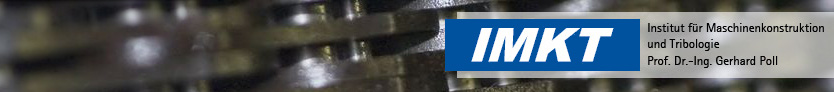
\includegraphics[width=\textwidth]{./images/imkt_logo_small.jpg}
    };

        \begin{scope}[x={(imkt.south east)}, y={(imkt.north west)}]
            %\draw[help lines, xstep=0.1, ystep=0.1] (0, 0) grid (1, 1);
            %\foreach \x in {0, 1, ..., 9} {
            %    \node [anchor=north] at (\x/10,0) {0.\x};
            %}
            %\foreach \y in {0, 1, ..., 9} {
            %    \node [anchor=east] at (0, \y/10,0) {0.\y};
            %}

            \node[anchor=south west, inner sep=0] (luh) at (0.05, 0.15) {
                
\includegraphics[width=4.7cm]{./images/luh_logo.png}
            };
        \end{scope}
\end{tikzpicture}

% ----------------------------------------
% Titel der Arbeit
% ----------------------------------------
\vspace{1cm}

\begin{center}
    \textbf{{\Large Entwicklung eines modularen Messsystems zur optischen und kapazitiven Schmierfilmdickenmessung in einem EHD-Kontakt}}
\end{center}

% ----------------------------------------
% Bild für diese Arbeit
% ----------------------------------------

% ----------------------------------------
% Masterarbeit und VW Logo
% ----------------------------------------
\vspace{12cm}

\begin{center}
    {\textbf{\Large Masterarbeit}}\\[1cm]

    {\large Durchgeführt bei der}

    {\large Volkswagen AG, Wolfsburg}

    
\includegraphics[width=2cm]{./images/vw_logo.png}
\end{center}

% ----------------------------------------
% Verfasser                     Betreuer
% ----------------------------------------
\vfill

\begin{minipage}[t]{0.5\textwidth}
    \begin{flushleft}
        Verfasser:

        cand. mach. Ngoc Minh \textsc{Dao}
    \end{flushleft}
\end{minipage}
%
\begin{minipage}[t]{0.5\textwidth}
    \begin{flushright}
        Betreuer:

        Dipl.-Ing. Norbert \textsc{Bader}
    \end{flushright}
\end{minipage}

% ----------------------------------------
% Seperate line
% ----------------------------------------
\rule{\textwidth}{1pt}

% ----------------------------------------
% Bericht Nr                    Ort, Datum
% ----------------------------------------
\begin{minipage}[t]{0.5\textwidth}
    \begin{flushleft}
        \textbf{Bericht Nr. 1412}
    \end{flushleft}
\end{minipage}
%
\begin{minipage}[t]{0.5\textwidth}
    \begin{flushright}
        \textbf{Hannover, \today}
    \end{flushright}
\end{minipage}


\restoregeometry

% ----------------------------------------
% Table of contents
% ----------------------------------------
\tableofcontents
%\listoffigures
%\listoftables
%\listoftodos[Notes]

% ----------------------------------------
% Nomenklatur
% ----------------------------------------
\addcontentsline{toc}{chapter}{Nomenklatur}
\chapter*{Nomenklatur}

\begin{longtable}{>{$}l<{$}cp{12cm}}
    \textbf{Symbol}  & \textbf{Einheit}                         & \textbf{Bezeichnung}                                         \\
    \midrule
    a                & \si{m}                                   & Halbachse der Kontaktellipse senkrecht zur Bewegungsrichtung \\
    b                & \si{m}                                   & Halbachse der Kontaktellipse parallel zur Bewegungsrichtung  \\
    C                & \si{\per\pascal}                         & Kompressibilität                                             \\
    E                & \si{\newton\per\meter^2}                 & Elastizitätsmodul                                            \\
    F                & \si{N}                                   & Normalkraft im Kontaktpunkt                                  \\
    G                & -                                        & Werkstoffparameter                                           \\
    H                & -                                        & Schmierfilmparameter                                         \\
    h                & \si{\meter}                              & Schmierfilmdicke                                             \\
    h_0              & \si{\meter}                              & Minimale Schmierfilmdicke (glatte Oberflächen)               \\
    n                & -                                        & Brechungsindex                                               \\
    P                & \si{N}                                   & Belastung im Kontakt                                         \\
    p                & \si{\pascal}                             & Druck im Kontaktpunkt                                        \\
    p_{0}            & \si{\pascal}                             & Maximaldruck im Kontaktpunkt                                 \\
    r                & \si{\meter}                              & Krümmungsradius der Kontaktkörper                            \\
    R                & \si{\meter}                              & Reziproker Krümmungsradius                                   \\
    R_{x}            & \si{\meter}                              & Hauptkrümmungsradius in der Bewegungsebene                   \\
    S                & -                                        & Schnittpunkt der Rotationsachsen                             \\
    S_{B}            & \si{\percent}                            & Bohrschlupf                                                  \\
    U                & -                                        & Geschwindigkeitsparameter                                    \\
    u                & \si[per-mode=symbol]{\meter\per\second}  & Wälzgeschwindigkeit im Schmierfilm                           \\
    W                & -                                        & Belastungsparameter                                          \\
    \alpha, \alpha^* & \si{\per\pascal}                         & Druck-Viskosität-Koeffizient                                 \\
    \beta            & \si{\per\kelvin}                         & Temperatur-Viskosität-Koeffizient                            \\
    \gamma           & \si{\per\second}                         & Schergefälle                                                 \\
    \gamma{_1}       & \si{\degree}                             & Neigungswinkel der Rotationsachse der Scheibe                \\
    \gamma{_2}       & \si{\degree}                             & Neigungswinkel der Rotationsachse der Kugel                  \\
    \eta             & \si{\pascal.\second}                     & Viskosität                                                   \\
    \eta{_0}         & \si{\pascal.\second}                     & Viskosität im Kontakteintritt ($p =$ \num{0})                \\
    \eta{_s}         & \si{\pascal.\second}                     & Viskosität beim Druck $p$ (Barus)                            \\
    \kappa           & -                                        & Verhältnis der Halbachsen der Kontaktellipsen                \\
    \nu              & -                                        & Querkontraktionszahl                                         \\
    \nu              & \si{m^2/s}                               & Kinematische Viskosität                                      \\
    \rho             & \si{kg/m^3}                              & Dichte                                                       \\
    \varphi          & \si{\degree}                             & Winkel zwischen den Hauptebenen                              \\
\end{longtable}%



% ----------------------------------------
% Einleitung
% ----------------------------------------
\chapter{Einleitung}
\label{chap:einleitung}



% ----------------------------------------
% Stand der Technik
% ----------------------------------------
% ----------------------------------------
% Chapter: Stand der Technik
% ----------------------------------------
\chapter{Stand der Technik}
\label{chap:stand_der_technik}

Ein geschmierter Reibungskontakt kann auf vier Elemente des tribologischen Systems nach Czichos \cite{czihos} reduziert werden:
\begin{itemize}
    \item Grundkörper
    \item Gegenkörper
    \item Zischenstoff
    \item Umgebungsmedium
\end{itemize}
% ----------------------------------------
% Fig: Das tribologische System
% ----------------------------------------
\begin{figure}[htb]
    \centering
    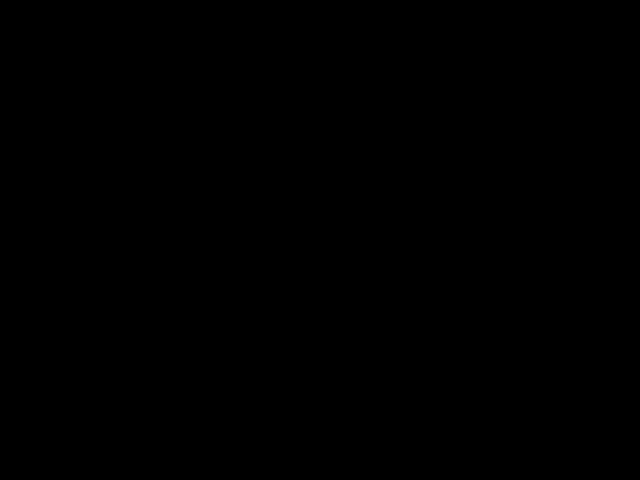
\includegraphics[width=5cm]{./images/blank_img.jpg}
    \caption{Das tribologische System}
    \label{fig:das_tribologische_system}
\end{figure}

Um ein besseres Verständnis der EHD-Schmierung zu haben, wird in diesem Abschnitt zuerst die Kennwerte des Zwischenstoffes (Schmiermittel) und der beiden Kontaktelementen (Grund- und Gegenkörper) ausführlich besprochen.
Danach wird der Mechanismus der EHD-Schmierung beleuchtet und am Ende wird die Arbeit von Hamrock und Dowson zur theoretischen Bestimmung der Schmierfilmdicke erwähnt.

% ----------------------------------------
% Sec: Eigenschaften des Schmiermittels
% ----------------------------------------
\section{Eigenschaften des Schmiermittels}
\label{sec:eigenschaften_des_schmiermittels}

Viskosität, die auch als innere Reibung bezeichnet wird, ist die wichtigste Kenngröße eines Schmierstoffes.
Sie beschreibt die Zähigkeit von Flüssigkeiten und Gasen.
Je größer die Viskosität ist, desto dickflüssiger ist das Fluid und je niedriger die Viskosität, desto dünnflüssiger ist es.
Ein Modell des Parallelplattenversuchs veranschaulicht das FließVerhalten des Schmierstoffes, Abbildung \ref{fig:geschwindigkeitsprofil_parallelplattenversuch}.
% ----------------------------------------
% Fig: Geschwindigkeitsprofil in einem Parallelplattenversuch
% ----------------------------------------
\begin{figure}[htb]
    \centering
    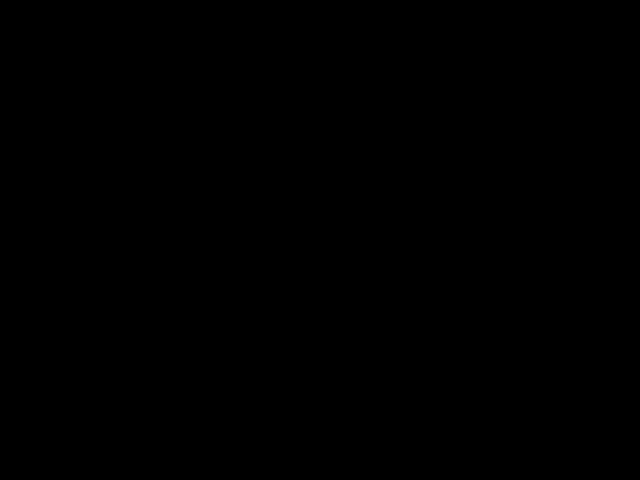
\includegraphics[width=5cm]{./images/blank_img.jpg}
    \caption{Geschwindigkeitsprofil in einem Parallelplattenversuch}
    \label{fig:geschwindigkeitsprofil_parallelplattenversuch}
\end{figure}

Für eine Newtonsche Flüssigkeit ist das Schergefälle $G = du/dz$ direkt proportional zur der Schubspannung $\tau$
% ----------------------------------------
% Eq: Schergefälle
% ----------------------------------------
\begin{equation}
    G = k \cdot \tau
    \label{eq:schergefaelle}
\end{equation}

Die dynamische Viskosität (oder Viskosität) ist das Verhältnis von Schubspannung und Geschwindigkeitsgradient und ist der Kehrwert der Fluidität $k$ im Newtonschen Schubspannungsgesetz (\ref{eq:schergefaelle}).
% ----------------------------------------
% Eq: Dynamische Viskosität
% ----------------------------------------
\begin{equation}
    \eta = \frac{1}{k} = \frac{\tau}{G} = \frac{\tau}{du/dz}
    \label{eq:dynamische_viskositaet}
\end{equation}

Die kinematische Viskosität ergibt sich aus der dynamischen Viskosität durch die Division mit der Dichte des Fluids.
% ----------------------------------------
% Eq: Dynamische Viskosität
% ----------------------------------------
\begin{equation}
    \nu = \frac{\eta}{\rho}
    \label{eq:kinematische_viskotitaet}
\end{equation}

Im Si-Einheitensystem hat die dynamische Viskosität als Einheit $N \cdot s/m^2$ oder $Pa \cdot s$ und die kinematische Viskosität als Einheit $m^2/s$.
Ein Stoff hat die Viskosität $1~N \cdot s/m^2$, wenn er in zwischen zwei Platten, die Größe von $1~m^2$ und einen Abstand von $1~m$ haben, befindet und man braucht $1~N$, um die zwei Platten gegeneinander mit einer Geschwindigkeit von $1~m/s$ zu verschieben.

Die Temperatur hat eine große Effekt auf der Viskosität aller fließfähigen Stoffe.
Mit steigender Temperatur sinkt die Viskosität der Flüssigkeiten ab.
Diese Effekt kann experimentell mittel eines Viskosimeters und rechnerisch nach Cameron bestimmt werden.

Die einfachste Gleichung nach Reynold lautet:
% ----------------------------------------
% Eq: Dynamische Viskosität nach Reynold
% ----------------------------------------
\begin{equation}
    \eta = \eta_{s} \cdot exp (-\beta \cdot \Delta\phi)
    \label{eq:dynamische_viskositaet_reynold}
\end{equation}
%
wobei $\eta_{s}$ ist die Viskosität des Schmierstoffes bei der Temperatur $\phi_{s}$, $\eta$ ist die Viskosität des Schmierstoffes bei der Temperatur $\phi$, $\Delta{\phi}$ ist die Temperaturdifferenz ($\eta = \eta_{s} + \Delta{\phi}$) und $\beta$ ist die thermoviskose Konstante.\improvement{check the formel}
% ----------------------------------------
% Eq: Dynamische Viskosität nach Cameron
% ----------------------------------------
\begin{equation}
    \eta(\phi) = k_1 \cdot exp \left( \frac{k_2}{\phi + 95} \right)
    \label{eq:dynamische_viskositaet_cameron}
\end{equation}
%

\begin{itemize}
    \item Viskosität
    \item Kinematische Viskosität
    \item Temperatureffekt
    \item Einfluss von Druck auf Viskosität
    \item Dichte
    \item Brechungsindex
    \item Wärmeleitfähigkeit
    \item Nichtnewtonsches Verhalten
    \item Verfestigung der Schmierung bei hohem Druck
\end{itemize}

% ----------------------------------------
% Sec: Betrachtung des EHD-Kontaktes
% ----------------------------------------
\section{Betrachtung des EHD-Kontaktes}
\label{sec:betrachtung_des_ehd_kontaktes}

\begin{itemize}
    \item Nichtkonformer Kontakt
    \item Hertzsche Gesetz
        \begin{itemize}
            \item Kugel-Kugel
            \item Kugel-Platte
        \end{itemize}
    \item Kontakt von beschichteten Körpern
\end{itemize}

% ----------------------------------------
% Sec: Elastohydrodynamische Schmiertheorie
% ----------------------------------------
\section{Elastohydrodynamische Schmiertheorie}
\label{elastohydrodynamische_schmiertheorie}

Erklärung, wie EHD funktioniert

% ----------------------------------------
% Sec: Schmierung nach Hamrock und Dowson
% ----------------------------------------
\section{Schmierfilmdicke nach Hamrock und Dowson}
\label{sec:schmierfilmdicke_nach_hamrock_und_dowson}
Erklärung, wie mann die Schmierfilmdicke berechnen kann



% ----------------------------------------
% Literaturforschung der experimentellen Technik in der EHD Schmierung
% ----------------------------------------
\chapter{Literaturforschung der experimentellen Technik in EHD Schmierung}
\label{chap:literaturforschung_der_experimentellen_technik_in_ehd_schmierung}
% ----------------------------------------
% Optische Methode
% ----------------------------------------
\section{Optische Messung der EHD Schmierfilmdicke}
\label{sec:optische_messung_der_ehd_schmierfilmdicke}

\subsection{Licht Interferometrie}
\label{ssec:licht_interferometrie}

\subsection{Messung der EHD Filmdicke}
\label{ssec:messung_der_ehd_filmdicke}

\subsection{Variante von der klassichen optischen Interferometrie Methode}
\label{ssec:variante_interferometrie}

% ----------------------------------------
% Elektrische Methode
% ----------------------------------------
\section{Elektrische Messung der EHD Schmierfilmdicke}
\label{sec:elektrische_messung_der_ehd_schmierfilmdicke}

\subsection{Kapazitive Methoden}
\label{ssec:kapazitive_methoden}

\subsection{Resistive Methoden}
\label{ssec:resistive_methoden}

% ----------------------------------------
% Alternative Methoden
% ----------------------------------------
\section{Alternative EHD Schmierfilmdicke Messmethoden}
\label{sec:alternative_messmethoden}

\subsection{Ultraschall}
\label{ssec:ultraschall}

\subsection{Laserinduzierte Fluoreszenz}
\label{ssec:laserinduzierte_fluoreszenz}


% ----------------------------------------
% Aufbau und Funktion des EHD-Messgeräts
% ----------------------------------------
% ----------------------------------------
% Chap: Aufbau und Funktion des EHD-Messgeräts
% ----------------------------------------
\chapter{Aufbau und Funktion des EHD-Messgeräts}
\label{chap:aufbau_und_funktion_des_ehd_messgeraets}

Zur Schmierfilmdickenmessung wurde ein ``EHL Ultra Thin Film Measurement System'' der Firma PCS-Instrument genutzt (siehe Abbildung~\ref{fig:ehl_messgeraet}).
Es basiert auf dem Kugel-Scheibe-Modell.
Mit optischer Interferenz wird die Schmierfilmdicke im EHD-Kontakt ermittelt.
Durch einen leicht modifizierten Aufbau ermöglicht das Gerät auch die Bestimmung von Reibkoeffizienten der eingesetzten Schmierstoffe.
Im Folgenden wird kurz auf die einzelnen Komponenten des EHL-Gerätes und die Modifikation im Rahmen dieser Arbeit eingegangen.

% ----------------------------------------
% Fig: EHL Prüfstand
% ----------------------------------------
\begin{figure}[htb]
    \centering
    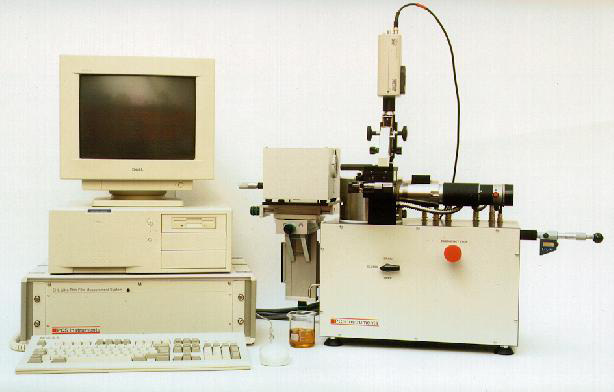
\includegraphics[width=0.8\linewidth]{./images/ehl_pruefstand.png}
    \caption{EHL-Messgerät~\cite{ehl}}
    \label{fig:ehl_messgeraet}
\end{figure}

% ----------------------------------------
% Sec: PC und Elektronikeinheit
% ----------------------------------------
\section{PC und Elektronikeinheit}
\label{sec:pc_elektronikeinheit}

Zur Bedienung des Prüfstands steht ein PC zur Verfügung.
Der PC hat Windows 98 als Betriebssystem und fünf ISA-Steckkarten.
Diese Karten sind für die Ein-/Ausgabe, die Zeiterfassung, die SW-Bilderfassung sowie ADC und DAC zuständig.
Die Kommunikation mit dem Prüfstand erfolgt durch das Softwarepaket ``Ultra Thin Film EHL Measurement''.
Der PC ist mit einem Spektrometer, einem SW-Monitor und einer Elektronikeinheit verbunden.

Zu der Elektronikeinheit gehören die Motoren, die Lasteinheit sowie die Heizvorrichtung.
Außerdem ist eine Überwachungsfunktion eingebaut, die bei einem Absturz der Software oder des PC den Prüfstand abschaltet.

% ----------------------------------------
% Sec: Meschanischer Aufbau
% ----------------------------------------
\section{Mechanischer Aufbau}
\label{sec:mechanischer_aufbau}

Abbildung~\ref{fig:ehl_aufbau} zeigt den Schematischen Aufbau des EHL-Prüfstands.
Das Reservoir ist bei Messungen mit Öl bis zur Hälfte der Kugel gefüllt.
Durch die Heizvorrichtung kann das Öl bis c.a \SI{150}{\degreeCelsius} erhitzt werden.

% ----------------------------------------
% Fig: EHL Aufbau
% ----------------------------------------
\begin{figure}[htb]
    \centering
    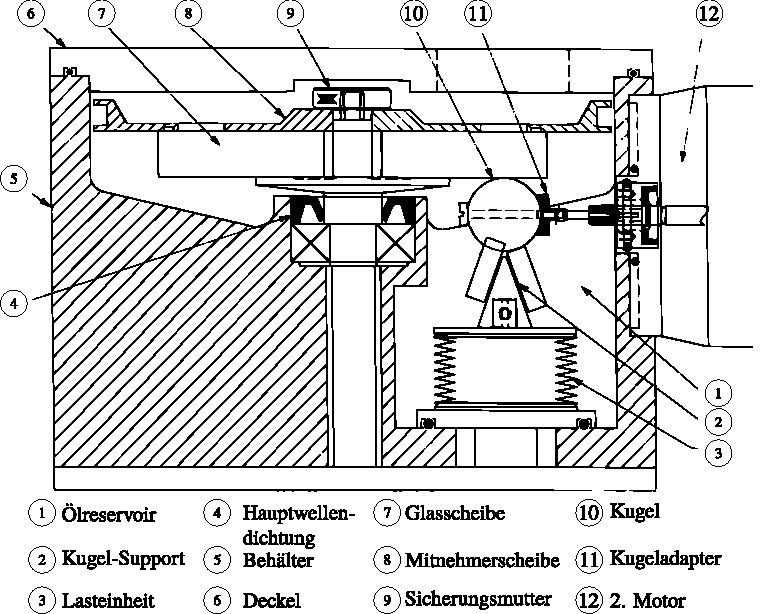
\includegraphics[width=0.8\textwidth]{./images/ehd_pruefstand_aufbau.pdf}
    \caption{Schematischer Aufbau des EHL-Prüfstands~\cite{ehl}}
    \label{fig:ehl_aufbau}
\end{figure}

Der elastohydrodynamische Schmierfilm wird durch einen Kugel-Scheibe-Kontakt erzeugt.
Die Kugel ist hochglanzpoliert, aus 100Cr6 Stahl und hat einen Durchmesser von \SI{19.05}{\milli\meter}.
Es gibt zwei Variationen der Kugel: normal und durchbohrt.
Über ein Kugel-Support wird die Kugel von unten von einer Lasteinheit gegen eine rotierende Glasscheibe gedrückt.
Die Last ist von \SIrange{0}{50}{\newton} wählbar und ergibt einen maximalen Druck von \SI{0.7}{\giga\pascal} im Kontaktpunkt (bei Glasscheibe).
Die Glasscheibe hat einen Durchmesser von \SI{100}{\milli\meter} und ist an der Unterseite mit einer durchlässigen Chromschicht und einer Silikatschicht versehen.
Es gibt durch die axiale Verschiebung des Kugel-Supports insgesamt \num{21} befahrbare Spuren ($R = 34 \rightarrow 44$ \si{\milli\meter}) auf der Scheibe.
Ein Spurwechsel ist nötig, weil die Silikatschicht, die nicht so robust wie die Chromschicht ist, im Laufe der Zeit abgenutzt wird.

Die Glasscheibe kann von \SI[per-mode=symbol]{1}{\milli\meter\per\second} bis \SI[per-mode=symbol]{5}{\meter\per\second} durch einen Motor betrieben werden.
Ein weiterer Motor ermöglicht auch das Antreiben der Kugel.
In diesem Fall sind Versuche mit Schlupf zwischen Kugel und Scheibe innerhalb von \SIrange{0}{200}{\percent} möglich.

Das originale Kugel-Support von PCS-Instrument besteht aus drei Lagern, die auf einem dreieckigen Aluminium-Klotz geschraubt werden.
Eine modifizierte Lagerung mit einstellbarer, geführter Achse von Wittek~\cite{wittek_2007} steht zudem zur Verfügung (siehe Abbildung~\ref{fig:kugel_support}).

% ----------------------------------------
% Fig: Kugel-Support
% ----------------------------------------
\begin{figure}[htb]
    \centering
    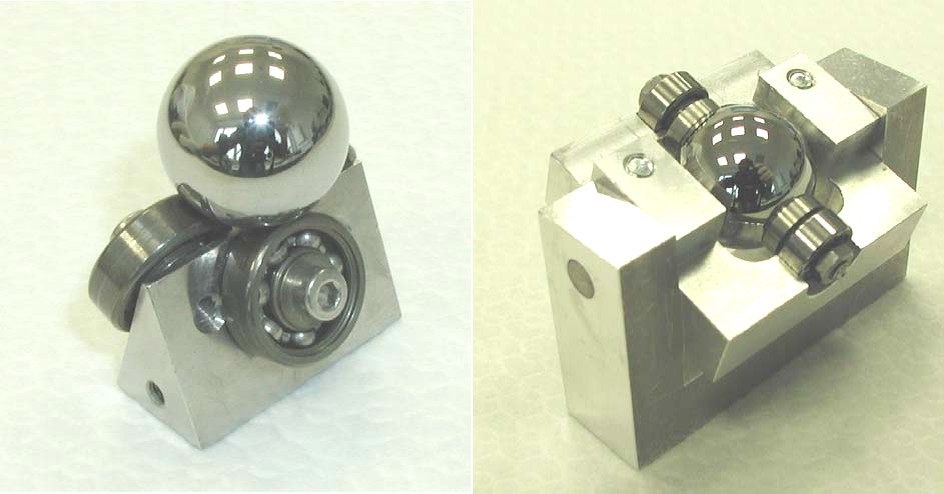
\includegraphics[width=0.6\textwidth]{./images/kugel-support_original_und_wittek.jpg}
    \caption{Originaler PCS-Support (links) und von \textit{Wittek} modifizierter Support (rechts)~\cite{wittek_2007}}
    \label{fig:kugel_support}
\end{figure}

Die Spezifikationen des Prüfstands von PCS sind in Tabelle \ref{tab:ehl_specs} zusammengefasst.

% ----------------------------------------
% Sec: Messsystem zur Schmierfilmdickemessung
% ----------------------------------------
\section{Messsystem zur Schmierfilmdickemessung}
\label{sec:messsystem_zur_schmierfilmdickemessung}

Beim EHD-Prüfstand von PCS Instrument wird die Schmierfilmdicke im Kugel-Scheibe-Kontakt mit Weißlichtinterferometrie (siehe Abschnitt~\ref{sec:optische_messung_der_ehd_schmierfilmdicke}) bestimmt.
Der Kontakt wird von oben durch die Glasscheibe beleuchtet und das reflektierende Bild wird von einem Spektrometer bewertet.
Die Messeinrichtung wird in Abbildung~\ref{fig:ehl_messprinzip} dargestellt.

% ----------------------------------------
% Fig: EHL Messeinrichtung
% ----------------------------------------
\begin{figure}[htb]
    \centering
    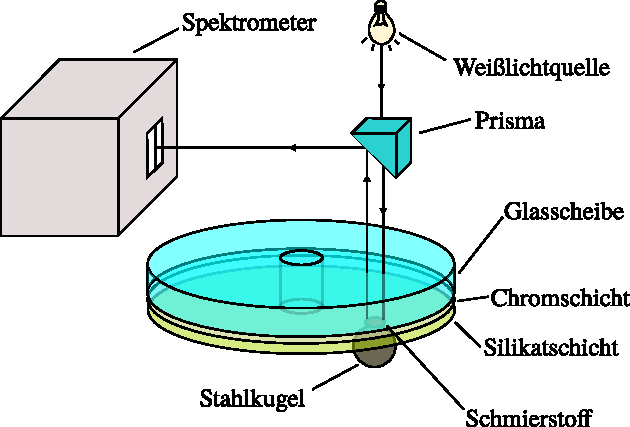
\includegraphics[]{./images/ehd_messprinzip.pdf}
    \caption{Messprinzip des EHD-Prüfstand von PCS~\cite{mach_2008}}
    \label{fig:ehl_messprinzip}
\end{figure}

Die Glasscheibe weist nicht nur eine Chromschicht, sondern auch eine Silikatschicht (Spacer-Layer) auf.
Diese hat die Funktion eines Harter-Ölfilms, der immer da ist.
Das heißt, dass es im Stillstand Interferenzen gibt.
Die Interferenzmuster sind fabelhafte Bilder (siehe Abbildung~\ref{fig:ehl_bilder}).
Aus ihrer Farben kann die Schmierfilmdicke bei bekannter Silikatschichtdicke berechnet werden.

% ----------------------------------------
% Fig: EHL Interferenzbilder
% ----------------------------------------
\begin{figure}[htb]
    \centering
    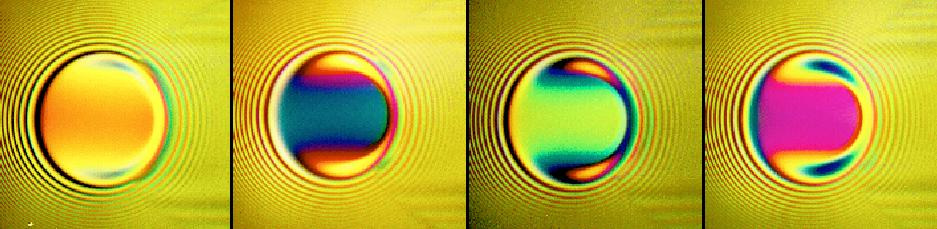
\includegraphics[width=0.8\textwidth]{./images/ehl_contact_at_increasing_speeds.png}
    \caption{Interferenzmuster eines Punktkontaktes bei zunehmenden Geschwindigkeiten~\cite{ehl_broshure}}
    \label{fig:ehl_bilder}
\end{figure}

Da eine Auswertung der Schmierfilmdicke aus den Farben der Interferenzen durch einen menschlichen Beobachter zu ungenau wäre, wird der reflektierende Lichtstrahl über ein Prisma durch einen Spalt in ein Spektrometer geleitet.
Dort werden die Interferenzmuster analysiert und aus einem SW-Monitor angezeigt (siehe Abbildung~\ref{fig:ehl_interferenzmuster}).

% ----------------------------------------
% Fig: EHL Beugungsmuster
% ----------------------------------------
\begin{figure}[htb]
    \centering
    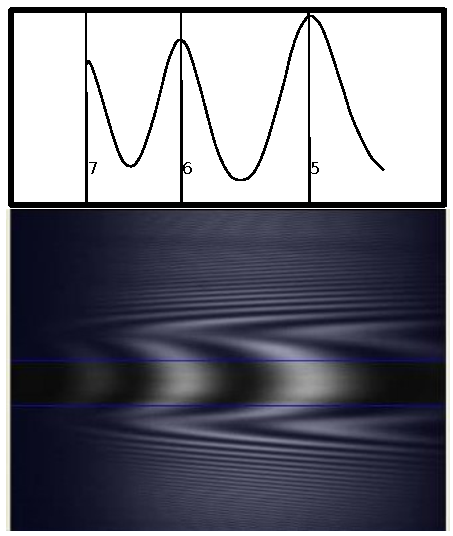
\includegraphics[]{./images/interferenzsmuster.pdf}
    \caption{Interferenzmuster im Spektrometer~\cite{ehl_broshure}}
    \label{fig:ehl_interferenzmuster}
\end{figure}

Der senkrechte, weiße Balken im Interferenzmuster sind die Maxima, wo die konstruktiven Interferenzen stattfinden und gibt die Wellenlänge an.
Wandern diese Balken nach rechts, nimmt die Wellenlänge bzw. Schmierfilmdicke zu.
Mit Hilfe des Ultra-Softwarepakets kann man aus dem Interferenzmuster die genaue Schmierfilmdicke berechnen.



% ----------------------------------------
% Konstruktive Bearbeitung
% ----------------------------------------
% ----------------------------------------
% Chap: Konstruktive Bearbeitung
% ----------------------------------------
\chapter{Konstruktive Bearbeitung}
\label{chap:konstruktive_bearbeitung}

Um die Messgenauigkeit der optischen Interferometrie-Technik mit der einfachen Adaptierbarkeit an verschiedenen realen Maschinenelementen der elektrischen Messmethode zur Schmierfilmdickenmessung im EHD-Kontakt zu vereinigen, soll ein neues modular Messsystem auf Basis des EHD-Prüfstands von PCS entwickelt werden.
Dies System soll die optische und elektrische (kapazitive) Messung gleichzeitig erlauben.
Für solches System gibt es die folgende Anforderungen, die durch konstruktive Bearbeitung in nächsten Abschnitten gelöst werden.
\begin{itemize}
    \item Elektrische Isolierung der Glasscheibe und der Kugel mit dem gesamten System.
    \item Elektrische Zugänge für die Messproben an der Scheibe und der Kugel.
    \item Beschichtung auf der Scheibe, die elektrische und optische Messung gleichzeitig erlaubt.
\end{itemize}

% ----------------------------------------
% Sec: Konstruktion der Kugelführung
% ----------------------------------------
\section{Konstruktion der Kugelführung}
\label{sec:konstruktion_der_kugelfuehrung}

Da das modifizierte Kugelsupport mit einstellbarer Achse von \textit{E. Wittek} \cite{wittek_2007} wegen Rundlaufabweichung nur bis Wälzgeschwindigkeit von c.a 0,7 $m/s$ einsetzbar ist, wird die originale Kugelführung der PCS Firma im Rahmen dieser Arbeit modifizierte und weiter benutzt.
Bei der standardmäßigen Kugelführung wird eine durchgebohrte Kugel in einem Adapter eingeklemmt, welche dann über einen Querstift mit der Motorausgangswelle des zweiten Antriebs formschlüssig verbunden wird.
Für die kapazitive Messung soll die Kugel elektrisch mit dem gesamten System isoliert werden, das erfolgt durch die Verwendung eine Kunststoffwelle.
Die Kugelaufnahme wird aus Messing gefertigt, um den Kontaktwiderstand mit den zu Signal übertragenden Kohlebürsten zu reduzieren.
Die Abbildung \ref{fig:aufbau_der_neuen_kugelfuehrung} zeigt den Zusammenbau der neuen Kugelführung.
% ----------------------------------------
% Fig: Aufbau der neuen Kugelführung
% ----------------------------------------
\begin{figure}[htb]
    \centering
    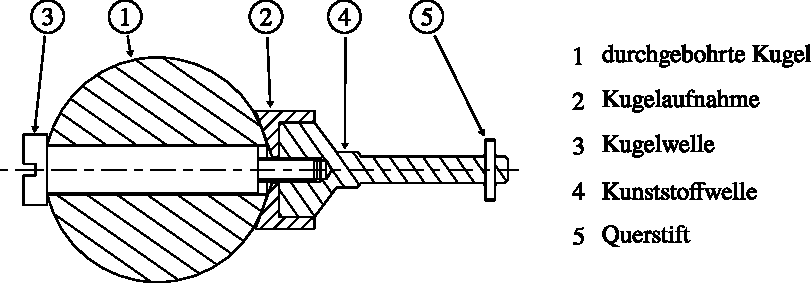
\includegraphics[]{./images/durchgebohrte_kugel.pdf}
    \caption{Aufbau der neuen Kugelführung}
    \label{fig:aufbau_der_neuen_kugelfuehrung}
\end{figure}
%

Die geführte Kugelachse ermöglicht die Versuche mit Schlupf und verhindert auch das unkontrollierte Einbringen des Schmierstoffes (Öl, Fett) in den Kontakt.
Der Kraftfluss zwischen dem zweiten Motor und der Kugel kann durch den Wegfall des Querstifts unterbrochen werden.
In diesem Fall dreht sich die Kugelführung frei in der Motorausgangswelle.

% ----------------------------------------
% Sec: Konstruktion des Kugelsupports
% ----------------------------------------
\section{Konstruktion des Kugelsupports}
\label{sec:konstruktion_des_kugelsupports}

Das neue Kugelsupport besteht aus drei Rillenkugellager, die durch drei $M3$ Schrauben auf einem dreieckigen Sockel befestigt werden (Abbildung \ref{fig:das_modifizierte_kugelsupport}).
Die Kugel wird von den drei Lagern sicher von unten gegen der Glasscheibe gestützt.
Da die Kugel mit der Lasteinheit elektrisch isoliert werden muss, wird der Sockel aus Kunststoff gefertigt.
Auf der Unterseite des Sockels befinden sich zwei Löcher, die mit den Stifte der Lasteinheit arretiert werden, dadurch wird die Position des Kugelsupports während Versuche sicher gestellt.
An der Seite des Sockels sind zwei M3 Bohrung zur Anbringung der Kohlebürstenhalter, die für die Aufnahme der elektrischen Signale von der Kugel zuständig sind, zu versehen.
Bei der Versuchen mit Fett ist dort auch möglich, die Befettungsvorrichtung zu montieren.
% ----------------------------------------
% Fig: Das modifizierte Kugelsupport
% ----------------------------------------
\begin{figure}[htb]
    \centering
    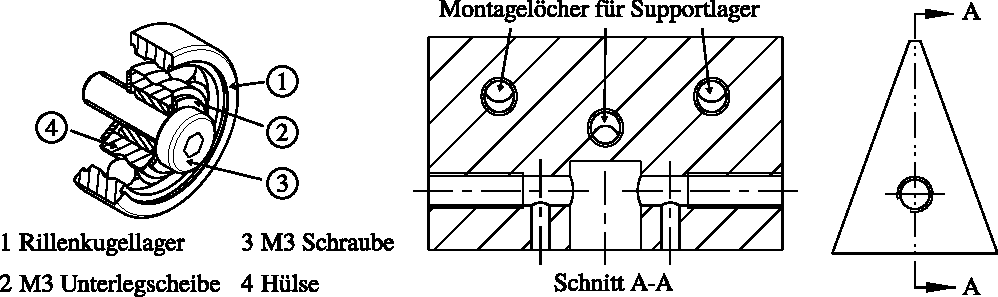
\includegraphics[]{./images/kugelsupport.pdf}
    \caption{Das Supportlager (links) und der Kunststoffsockel (rechts)}
    \label{fig:das_modifizierte_kugelsupport}
\end{figure}
%

Der Kohlebürstenhalter ist aus Messing, hat eine zylindrische Form und wird mit einem Blechhalter, welcher an der Seite des Supports angeschraubt wird, gelötet.
Die Kohlebürste Typ \textit{KK399} wurden von der Firma \textit{Schmidthammer} gekauft.
Dank dem hohen Kupferanteil (98\%) hat sie sehr geringen Kontaktwiderstand bzw. Eigenwiderstand.
Sie hat am Ende eine Kupferlitze und ist an anderen Seite mit Laufschräge zu versehen.
Leider ist die Laufschräge für diese Anwendung nicht geeignet und wurden flach geschliffen.
Die Kohlebürste wird von einer Feder (Typ \textit{LG860}) gegen der Lauffläche (Kugelaufnahme) gedrückt.
Abbildung \ref{fig:die_baugruppe_des_kohlebuerstenhalters} zeigt die Baugruppe des Kohlebürstenhalters.
% ----------------------------------------
% Fig: Blechhalter + Kohlebürstenhalter + Kohlebürsten + Feder
% ----------------------------------------
\begin{figure}[htb]
    \centering
    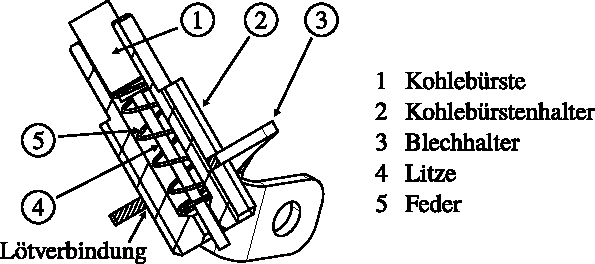
\includegraphics[]{./images/kohlebuerstenhalter_asm.pdf}
    \caption{Die Baugruppe des Kohlebürstenhalters}
    \label{fig:die_baugruppe_des_kohlebuerstenhalters}
\end{figure}
%

Um der elektrische Kontakt zwischen der Kugel und der Messprobe während der Versuche geringe Störungen zu halten, sind zwei Kohlebürsten für die Kugel zu versehen.
Abbildung \ref{fig:das_komplette_kugelsupports} zeigt das komplette Supports mit der neuen Kugelführung.
% ----------------------------------------
% Fig: Zusammenbau des gesamten Kugelsupports
% ----------------------------------------
\begin{figure}[htb]
    \centering
    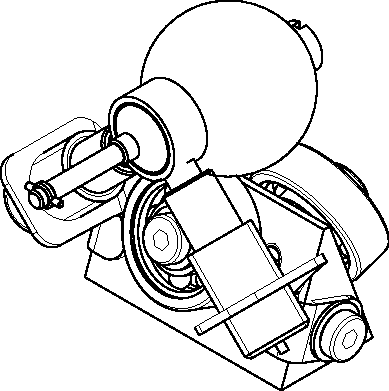
\includegraphics[]{./images/kugelsupport_full.pdf}
    \caption{Zusammenbau des neuen Supports mit der Kugel}
    \label{fig:das_komplette_kugelsupports}
\end{figure}
%

% ----------------------------------------
% Sec: Die Glasscheibebaugruppe
% ----------------------------------------
\section{Die Glasscheibebaugruppe}
\label{sec:die_glasscheibebaugruppe}

Um die elektrische Messung bei dem vorhandenen Prüfstand durchzuführen, müssen die folgende Maßnahmen gemacht werden:
\begin{itemize}
    \item Stromleitende Beschichtung für die Glasscheibe
    \item Isolierung der Glasscheibe mit dem gesamten Prüfsystem
    \item Elektrischer Zugang für die Messprobe zur Unterseite der Glasscheibe
\end{itemize}

Wie im vorherigen Kapitel \ref{chap:literaturforschung_der_experimentellen_technik_in_ehd_schmierung} schon erwähnt, ist es auch möglich, die Schmierfilmdickenmessung bei einer Chrom beschichteten Scheibe durch zu führen.
Allerdings es gibt folgende Probleme bei der klassischen Messmethode.
Ersten bietet dieses Verfahren eine niedrige Auflösung. Zweiten ist eine monochrom Lichtquelle notwendig, es fehlt bei dem vorhandenen Prüfstand diesen Apparat.
Nicht zuletzt ist das \textit{Ultra-Softwarepaket} von PCS nicht in der Lager solche Messung durchzuführen bzw. auszuwerten.
Letzten ist der Eigenwiderstand der Chromschicht wegen ihrer extrem dünnen Dicke sehr hoch (größer als $1 k\omega$) und unregelmäßig verteilt.
\label{chap:literaturforschung_der_experimentellen_technik_in_ehd_schmierung}
Das macht die optische und elektrische Messung bei der Chrom-Glasscheibe ungünstig.

Eine andere Option ist die \textit{Spacer-Layer-Scheibe} zu benutzen.
Da die Silikatschicht nicht Strom leitend ist, wird die Hälfte der Scheibe mit einer dickeren Chromschicht (c.a $300 nm$) beschichtet (Abbildung \ref{fig:die_neu_beschichtet_glassscheibe}).
Durch die Erhöhung der Beschichtung wird der Eigenwiderstand reduziert und auch besser auf der Oberfläche verteilt.
Die unbehandelte Hälfte kann man wie normal mit der \textit{Spacer-Layer-Methode} die Schmierfilmdicke bestimmen.
% ----------------------------------------
% Fig: Bild der neuen beschichteten Scheibe
% ----------------------------------------
\begin{figure}[htb]
    \centering
    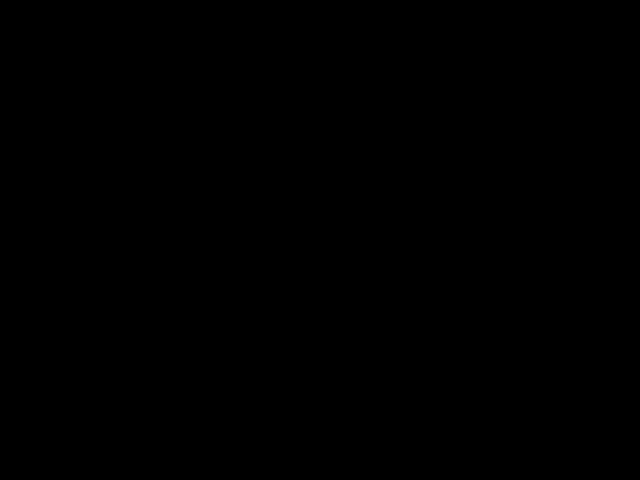
\includegraphics[width=4cm]{./images/blank_img.jpg}
    \caption{Die neu beschichtete Glasscheibe}
    \label{fig:die_neu_beschichtet_glassscheibe}
\end{figure}
%

Der nächste Schritt ist die behandelte Glasscheibe mit dem gesamten Testsystem isolieren.
Das erfolgt durch die Verwendung einer Kunststoff-Unterlegscheibe und einer Kunststoffhülse, die Unterseite der Scheibe mit der Welle des 1. Motors trennen (Abbildung \ref{fig:isolierung_der_glassscheibe})
% ----------------------------------------
% Fig: Isolierung der Scheibe
% ----------------------------------------
\begin{figure}[htb]
    \centering
    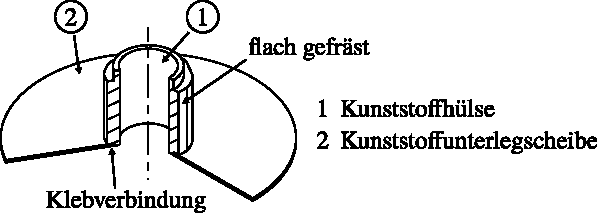
\includegraphics[]{./images/isolierung_der_scheibe.pdf}
    \caption{Isolierung der Glasscheibe}
    \label{fig:isolierung_der_glassscheibe}
\end{figure}
%

Beide Teile sind aus \textit{Polypropylen}, welcher bis $80 ^\circ C$ beständig ist und die Unterlegscheibe ist nur $0,5 mm$ dick.
Da die Lasteinheit nicht nur in die horizontale sondern auch in die vertikale Richtung sich bewegen kann, ist diese minimale Höheänderung der Glasscheibe kein Problem.
Die äußere Oberfläche der Hülse wurden an sechs Positionen flach gefräst. Die bilden sich mit der inneren Bohrung der Glasscheibe sechs Kanäle, die den Platz für die elektrische Verbindungen von Unterseite zur Oberseite der Scheibe schaffen.
Die Kunststoff-Unterlegscheibe wurde mit der Hülse mit dem \textit{Plastix} Klebe von Pattex geklebt, diese Verbindung ist gegen dem Wegrutschen der beiden Teilen während Betriebs zu sichern.

Um die elektrische Verbindung von der Unterseite der Scheibe nach oben zu bringen, werden sechs Kupferstreifen verwendet.
Sie werden auf der Kunststoff-Unterlegscheibe angeklebt und durch die sechs Kanäle (zwischen Hülse und Glasscheibe) nach oben geführt.
Dort werden sie bei der Montageposition zwischen der Oberkante der Hülse und einer Mitnehmerscheibe geklemmt und dadurch ist die elektrische Verbindung zwischen beiden Seite Scheibe hergestellt.
Die von oben geschraubt Sicherungsmutter sichert die ganze Baugruppe fest.
Die Abbildung \ref{fig:glasscheibebaugruppe} zeigt die ganze Baugruppe der Glasscheibe an.
% ----------------------------------------
% Fig: Glasscheibebaugruppe
% ----------------------------------------
\begin{figure}[htb]
    \centering
    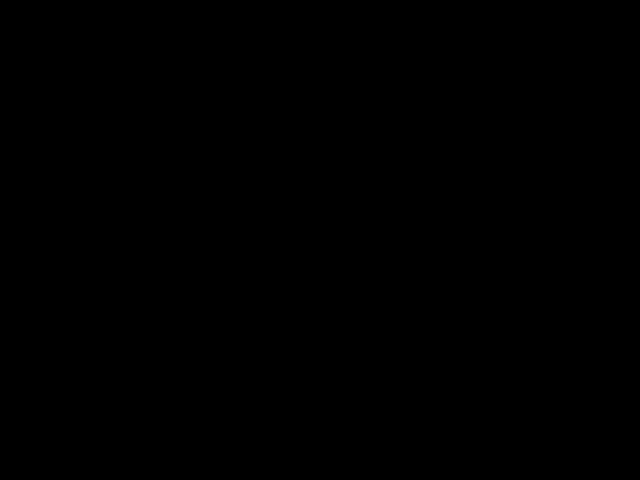
\includegraphics[width=4cm]{./images/blank_img.jpg}
    \caption{Glasscheibebaugruppe}
    \label{fig:glasscheibebaugruppe}
\end{figure}
%

% ----------------------------------------
% Sec: Konstruktion des Deckels
% ----------------------------------------
\section{Konstruktion des Deckels}
\label{sec:konstruktion_des_deckels}


% ----------------------------------------
% Versuche beim EHD-Messgerät
% ----------------------------------------
% ----------------------------------------
% Chap: Versuche auf dem EHD-Messgerät
% ----------------------------------------
\chapter{Versuche auf dem EHD-Messgerät}
\label{chap:versuche_auf_dem_ehd_messgeraet}

Um die Schmierfilmdicke im EHD-Komtakt mittels elektrischen Verfahrens zu bestimmen, braucht man die Kenntnis der dielektrischen Eigenschaften des Schmierstoffes, deren Abhängigkeit von der Temperatur, dem Druck.

% ----------------------------------------
% Sec: Bestimmung der Dielektrizitätskonstante
% ----------------------------------------
\section{Dielektrizitätskonstante des Schmierstoffes}
\label{sec:dielektrizitaetskonstate_des_schmierstoffes}


Die Bestimmung der Dielektrizitätskonstante des Öls \textit{FVA 3} wurde an einem kapazitiven Wegmessgerät durchgeführt.
Das Messgerät besteht aus zwei Stahlbacken, die auf einem Gestell aufgehängt werden, einem Zylinder und der elektronischen Einheit (siehe Abbildung \ref{fig:das_kapazitive_wegmessgeraet}).

% ----------------------------------------
% Fig: Kapazitiv Wegmessgerät beim IMKT
% ----------------------------------------
\begin{figure}[htb]
    \centering
    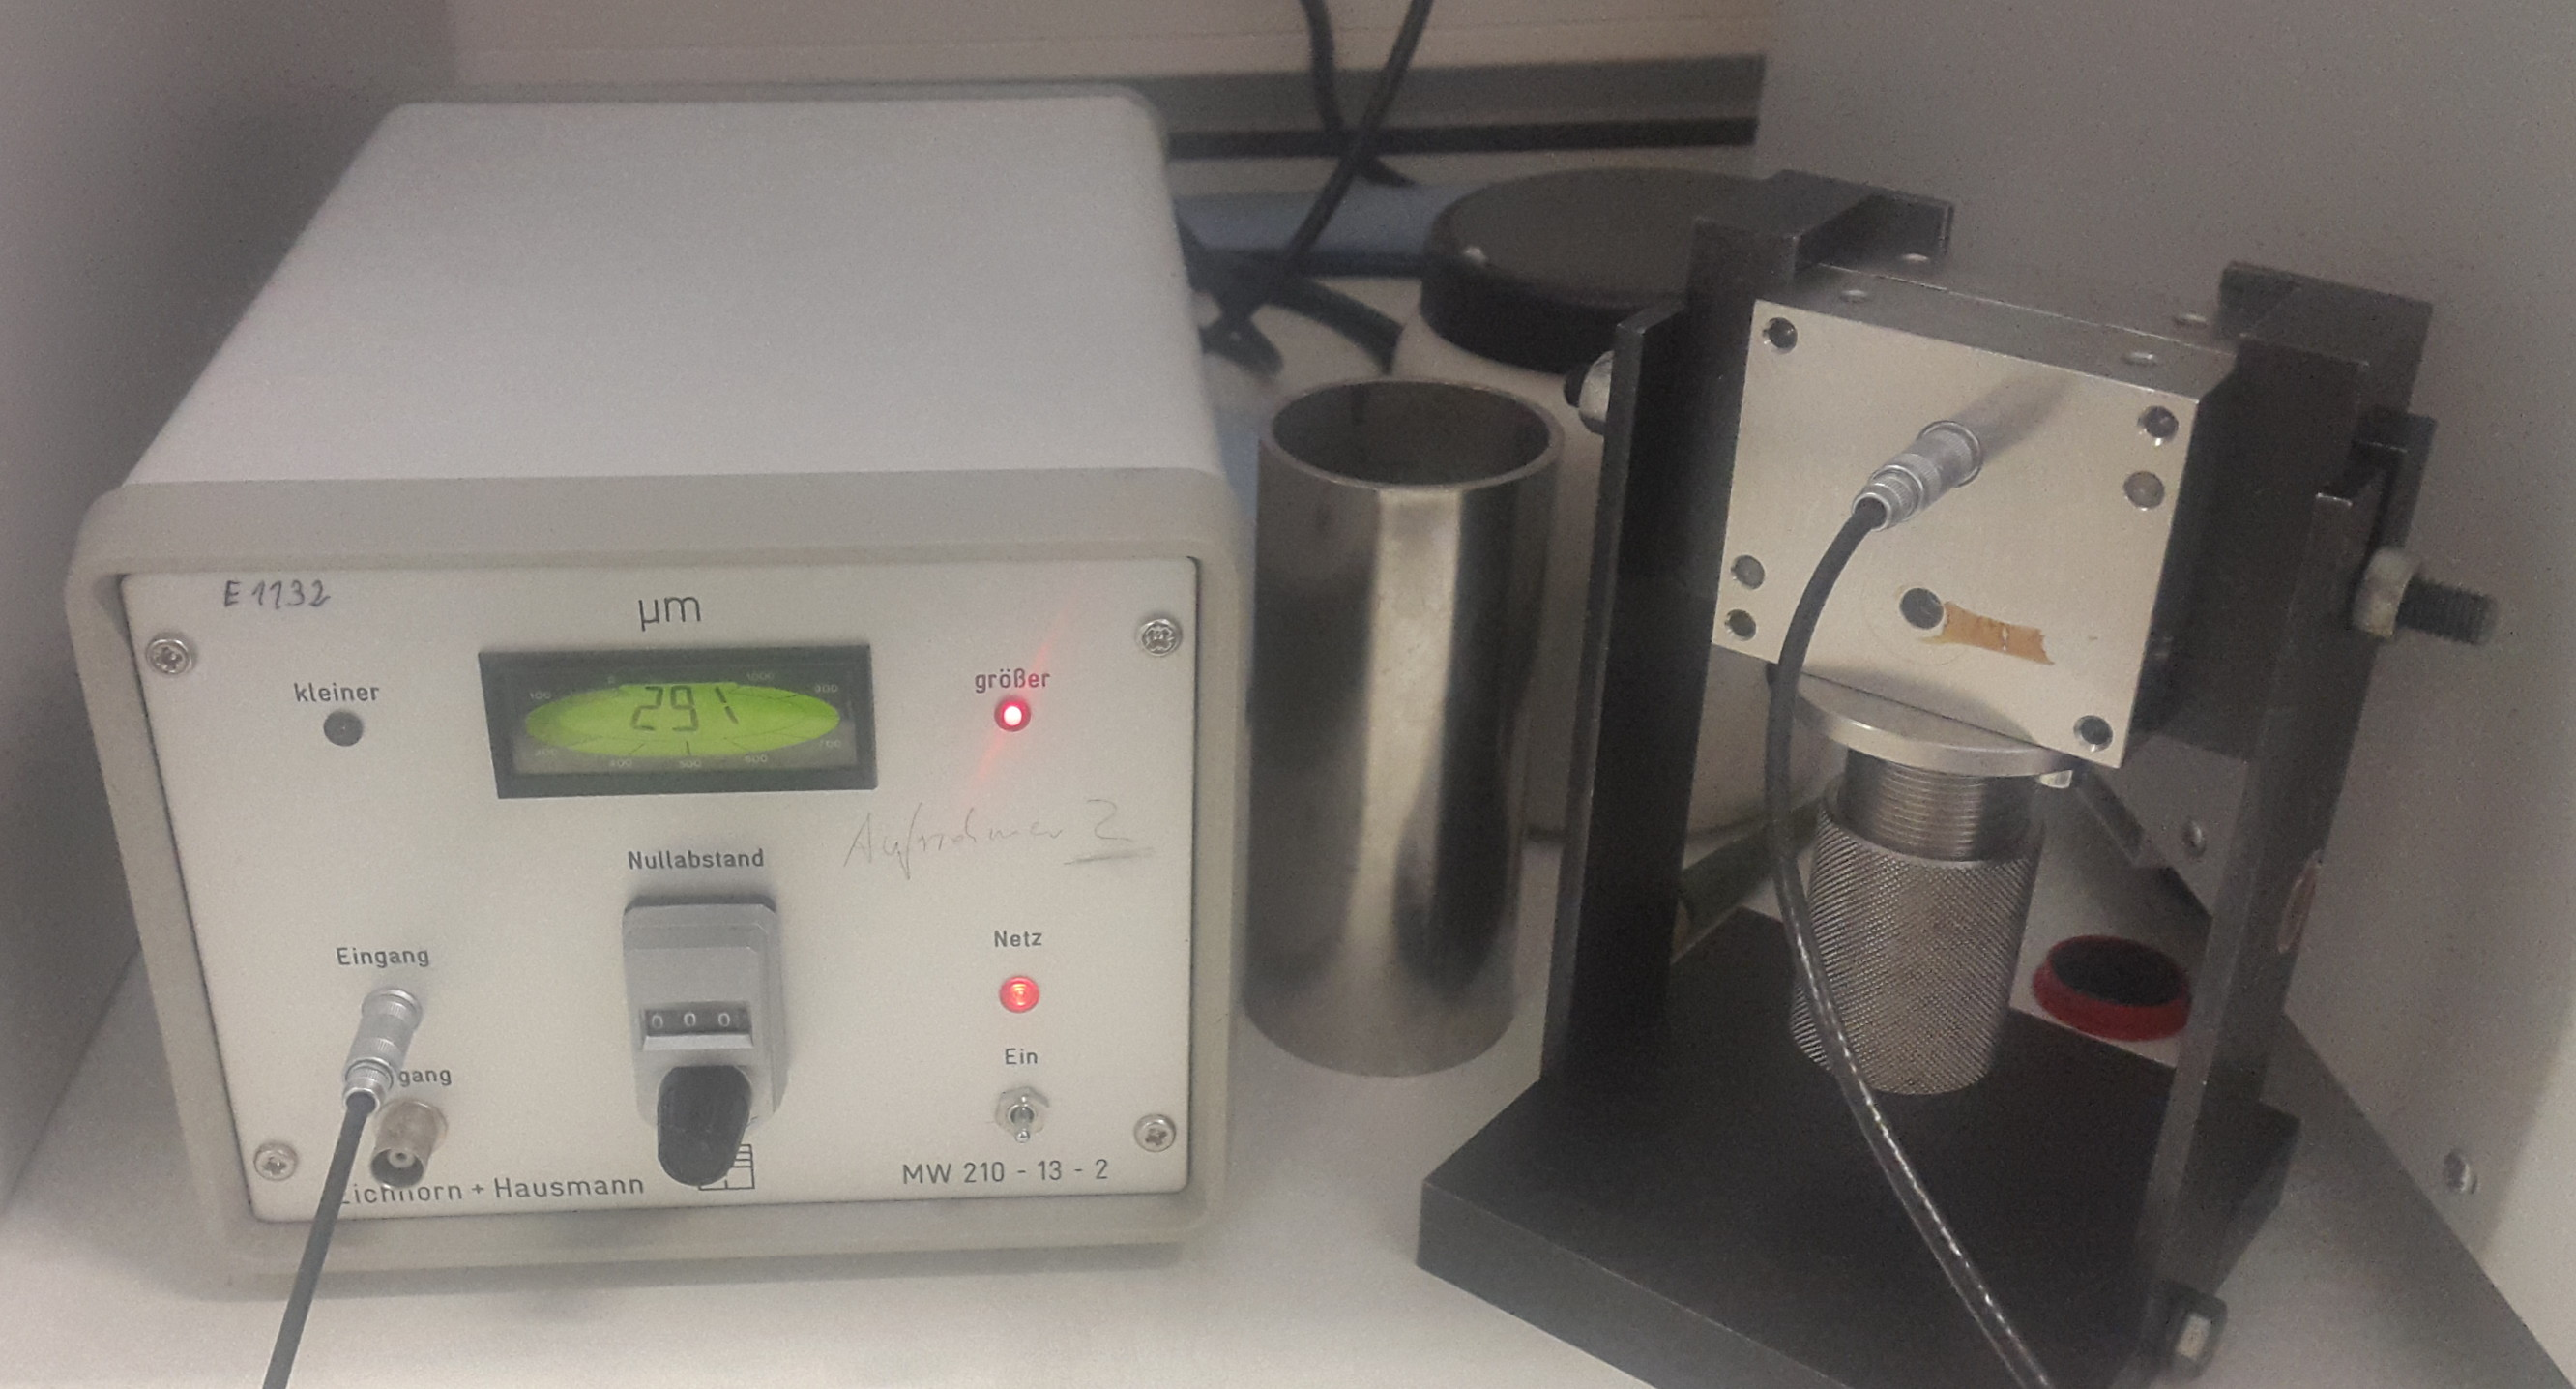
\includegraphics[]{./images/wegmessgeraet_imkt.pdf}
    \caption{Das kapazitive Wegmessgerät zur Bestimmung der Dielektrizitätskonstante des \textit{FVA 3} Öl}
    \label{fig:das_kapazitive_wegmessgeraet}
\end{figure}

Abbildung \ref{fig:wegmessgeraet_pruefkopf} zeigt den Prüfkopf des Wegmessgeräts im abgebauten Zustand.
An einem Backen befindet sich den Wegsensor, welcher bündig mit der Innenseite des Backen sitzt.
Bei dem anderen Backen wurde eine Nut auf der inneren Oberfläche gebracht, so dass, wenn beide Backen zusammen verschraubt werden, bildet sich einen Spalt in zwischen.
Der Zylinder wird an der unteren Seite den Backen angeflanscht.
Durch das Drehen der Mutter wird den Kolben nach oben gedrückt, damit wird das Öl in den Spalt gepumpt.

% ----------------------------------------
% Fig: Funktionsprinzip des Prüfkopfs des Messgeräts
% ----------------------------------------
\begin{figure}[htb]
    \centering
    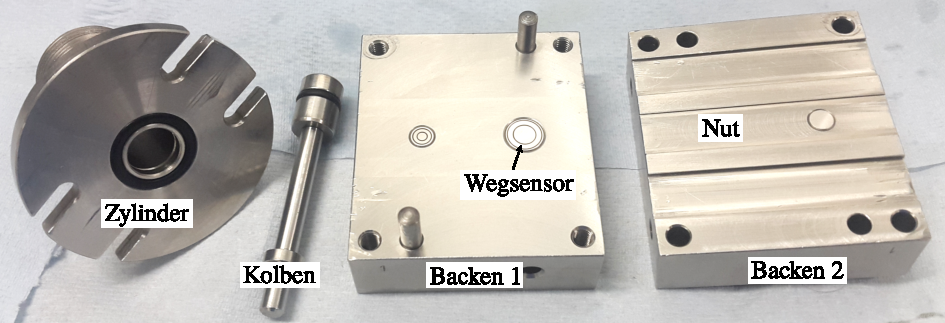
\includegraphics[]{./images/wegmessgeraet_pruefkopf.pdf}
    \caption{Der abgebaute Prüfkopf des Wegmessgeräts}
    \label{fig:wegmessgeraet_pruefkopf}
\end{figure}

Die Messung der Höhe des Spalts zwischen den Backen erfolgt durch die Betrachtung ihn als ein Plattenkondensator, welcher die Luft als Dielektrikum hat (Abbildung \ref{fig:plattenkondensator}).
Bei dem Einfordern des Öls in den Spalt ändert sich das Dielektrikum von Luft zu Luft + Öl, damit verändert sich seine Kapazität bzw. der Messwert, obwohl der Abstand im Spalt konstant bleibt.
Durch dies Phänomen wird die Dielektrizitätskonstante des Öls als das Verhältnis zwischen den Messwegen bei Luft und beim Öl berechnet.
Die Messergebnisse für das Öl \textit{FVA 3} bei verschiedenen Temperatur \SIrange{20}{80}{\degreeCelsius} werden in der Tabelle \ref{tab:relative_permittivitaet_fva3} dargestellt.

% ----------------------------------------
% Tab: Permittivität des FVA 3 Ols
% ----------------------------------------
\begin{minipage}[b]{0.55\linewidth}
    \centering
    \begin{tabular}{lrrr}
    Medium  & Temp [\si{\degreeCelsius}] & Weg [\si{\um}] & rel. Permittivität \\
    \hline
    Luft    & 20                         & 292            & 1                  \\
    FVA 3   & 40                         & 141            & 2.070              \\
    FVA 3   & 60                         & 142            & 2.056              \\
    FVA 3   & 80                         & 144            & 2.027              \\
    SHC 320 & 40                         & 118            & 2.474              \\
    SHC 320 & 60                         & 120            & 2.433              \\
    SHC 320 & 80                         & 122            & 2.393              \\
\end{tabular}

    \captionof{table}{relative Permittivität von \textit{FVA 3} bei unterschiedlichen Temperaturen}
    \label{tab:relative_permittivitaet_fva3}
\end{minipage}
\hspace{0.5cm}
%
% ----------------------------------------
% Fig: Plattenkondensator
% ----------------------------------------
\begin{minipage}[b]{0.3\linewidth}
    \centering
    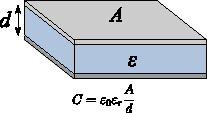
\includegraphics[width=\textwidth]{./images/plattenkondensator.pdf}
    \captionof{figure}{Plattenkondensator \cite{kondensator_wiki}}
    \label{fig:plattenkondensator}
\end{minipage}

% ----------------------------------------
% Sec: Kapazitive Messgeräte zur Schmierfilmdickenbestimmung
% ----------------------------------------
\section{Kapazitive Messgeräte zur Schmierfilmdickenbestimmung}
\label{sec:kapazitive_messgeraete_zur_schmierfilmdickenbestimmung}

% ----------------------------------------
% Sub: Stromladekurve Messgerät
% ----------------------------------------
\subsection{Stromladekurve Messgerät}
\label{sub:stromladekurve_messgeraet}

Im IMKT gibt es ein mobiles Messsystem zur Schmierfilmdickenmessung mittels kapazitiven Messverfahren.
Das System besteht aus einem Laptop, der mit \textit{Laderkurve-Software} installiert, und einer Messkarte (Typ USB-6211) von der Firma National Instrument (NI).

Bei kapazitiver Messmethode wird der EHD-Kontakt als ein Kondensator ($C_K$) betrachtet.
Die Auflade des Kondensators erfolgt durch eine Ladespannung $U_L$ (\SIrange{0,2}{0,5}{\volt}) und einen Vorwiderstand $R_V$ (\SI{1012.7}{\kilo\ohm}).
Eine unendliche Erhöhung der Ladespannung ist aber unerwünscht, weil die zur Ionisierung des Schmierstoffes bei hohen Spannung verursacht und das kann die Messergebnisse verfälschen.
Abbildung \ref{fig:Schematischer_aufbau_des_mobilen_messsystems} zeigt das Prinzip des mobilen Messsystems zur Schmierfilmdickenmessung bei IMKT an.
% ----------------------------------------
% Fig: Schematischer Aufbau des mobilen Messsystems
% ----------------------------------------
\begin{figure}[htb]
    \centering
    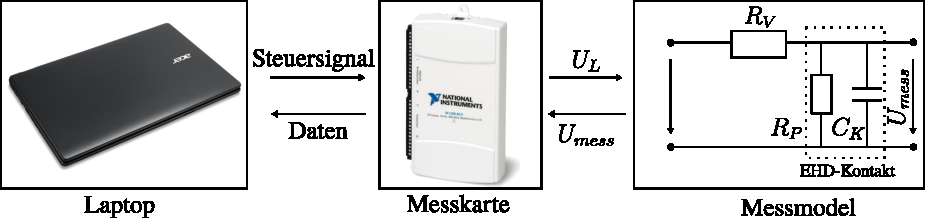
\includegraphics[]{./images/schematischer_aufbau_des_mobilen_messsystem.pdf}
    \caption{Schematischer Aufbau des mobilen Messsystems}
    \label{fig:Schematischer_aufbau_des_mobilen_messsystems}
\end{figure}

Das ganze Messsystem wird von der \textit{Laderkurve-Software} gesteuert.
Sie miss nicht direkt die Kapazität, sondern nimmt sie die Antwort bzw. Ladekurve des ``Kondensators'' auf, danach wird die Auswertung mit einem Matlab-Skript ausgeführt.
Die Software kann die Ladekurve in zwei Modi: \emph{Anzahl der Messwerte} oder \emph{Messung nach Zeit} aufnehmen.
Im Rahmen dieser Arbeit werden alle Messungen mit dem ersten Modus gemacht.
Abbildung \ref{fig:gui_der_laderkurve_software} zeigt die Benutzeroberfläche der Ladekurve-Software bei einer Testmessung mit einem Referenz-Kondensator (\SI{3.3}{\nano\farad}) an.
% ----------------------------------------
% Fig: GUI der Ladekurve-Software
% ----------------------------------------
\begin{figure}[htb]
    \centering
    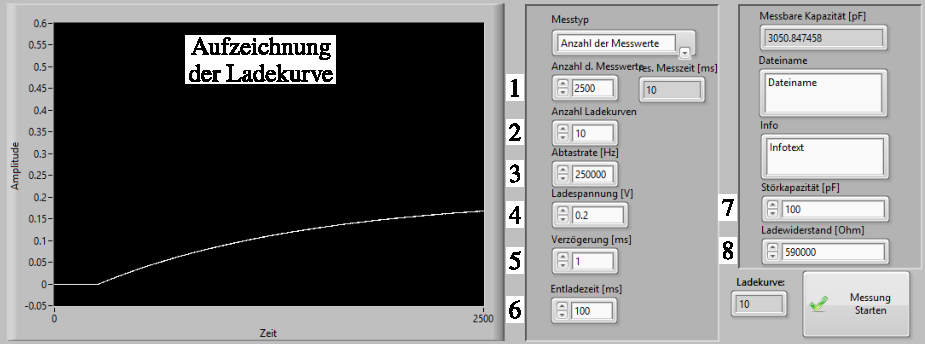
\includegraphics[]{./images/ladekurven_gui.pdf}
    \caption{Benutzeroberfläche der Laderkurve-Software}
    \label{fig:gui_der_laderkurve_software}
\end{figure}

Die Software ist relative einfach zu bedienen, allerdings gibt es folgende Punkte, auf die man beachten muss.
\begin{description}
    \item[1. Anzahl der Messwerte] ist die Auflösung der Messung.
        Zu niedriger Wert kann zum Messfehler führen und zu hohen Wert kann es schnell den Speicher voll machen, außerdem ist sie auch von der Abtastrate der Messkarte beschränkt.
        Der Standardwert ist \num{2500}.

    \item[2. Anzahl der Ladekurven] ist die Anzahl der Messungen, die nach einander durchgeführt werden. ist die Anzahl der Messungen, die nach einander durchgeführt werden.
        Der Standardwert ist \num{10}.

    \item[3. Abtastrate] ist die Anzahl der Messwerte, die Messkarte pro Sekunde messen kann.
        Die USB-6211 Messkarte von NI kann maximal \SI[per-mode=symbol]{250}{\kilo\sample\per\second}, das entspricht \num{2500} Messwerte in einem Zeitraum von \SI{10}{\milli\second}.

    \item[4. Ladespannung] ist die Spannung zwischen zwei Terminal des Kondensators.
        Der Wert sollte im Bereich von \SIrange{0.2}{0.5}{\volt} liegen.

    \item[5. Verzögerung] ist die Wartezeit, die die Software warten muss, bevor sie eine Messung ausführt.
        Der Standardwert ist \SI{1}{\ms}.

    \item[6. Entladezeit] ist die Zeit zwischen zwei Messungen.
        Sie ist notwendig, um der Kondensator komplette leer bevor jeder neuen Messung zu entladen.
        Der Standardwert ist \SI{100}{\ms}.

    \item[7. Störkapazität] ist die externe Störung, wie zum Beispiel von Messkabel oder statische Kapazität zwischen Messkörpern.

    \item[8. Ladewiderstand] ist der Wert des Vorwiderstands.
        Er ist nur für den Dokumentationszweck und wird in der Messdatei geschrieben.
        Dieser Wert wird für die spätere Auswertung verwendet.

    \item[9. Austecken des Netzteils] ist notwendig, um die Störungen von anderen elektronischen Geräte zu vermeiden.
\end{description}

%
% ----------------------------------------
% Sub: LCR Messgerät
% ----------------------------------------
\subsection{LCR Messgerät}
\label{sub:lcr_messgeraet}

In der Praxis kann jede Flüssigkeit und jeder Feststoff Strom durchlassen.
Wenn das Material von einem Wechselstrom gespeist wird, wird das Verhältnis zwischen der Spannung und dem Strom als Impedanz bezeichnet.
Die Veränderung der gemessenen Impedanz durch die Variation der Stromfrequenz ist von der Eigenschaft des Materials abhängig.
Das kann auf die physikalische Struktur des Werkstoffes, auf die innere chemische Prozesse oder eine Kombination von beiden zurückführen.
Der Zusammenhang zwischen der Impedanz, der Frequenz und der Kapazität von einem mit Wechselstrom angelegten Kondensators wird in der Formel \ref{eq:impedanz_kondensator} \cite{impedance} dargestellt.
%
\begin{equation}
    Z_{C} = \cfrac{v_C(t)}{i_C(t)} = \cfrac{1}{j \omega C}
    \label{eq:impedanz_kondensator}
\end{equation}

Im Gegenteil zum mobilen Ladekurve-Messsystem, welches die Kapazität über die Antwort einer Ladespannung interpretiert, bietet das LCR-Messgerät ST2826 der Firma Sourcetronic die Möglichkeit, die Kapazität eines EHD-Kontakts direkt zu messen.
Abbildung \ref{fig:versuchsaufbau_zur_kapazitaetsmessung_mit_lcr_meter} zeigt den Aufbau des Messsystems mit dem LCR-Messgerät.
% ----------------------------------------
% Fig: Schematischer Aufbau des Messsystems mit LCR-Meter
% ----------------------------------------
\begin{figure}[htb]
    \centering
    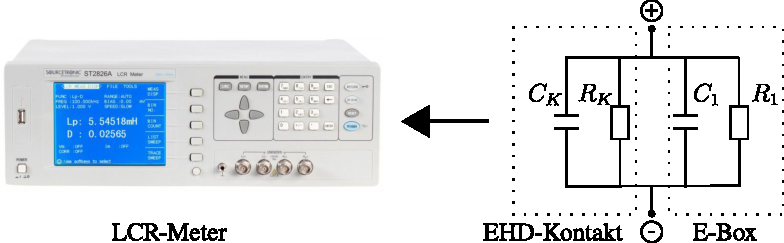
\includegraphics[]{./images/versuchsaufbau_mit_lcr_meter.pdf}
    \caption{Versuchsaufbau zur Kapazitätsmessung mit LCR-Meter}
    \label{fig:versuchsaufbau_zur_kapazitaetsmessung_mit_lcr_meter}
\end{figure}

Das LCR-Messgerät bietet einen breiten Frequenzbereich von \SI{20}{\Hz} bis \SI{50}{\MHz}.
Dank der Kelvin-Messproben (4-Punkt Messung) hat das Gerät eine sehr gute Genauigkeit von \SI{0.1}{\percent} und ermöglicht die Messung auch bei kleinsten Änderung des Systems.
Mit einer Sinuskorrelationstechnik bietet das Gerät eine rauschfreie Analyse.
Die Addition des Widerstands $R_1$ und des Kondensators $C_1$ sind benötigt, um zu sehen, ob der Strom tatsächlich durch den EHD-Kontakt fließt oder in irgeneiner Verbindung verloren geht.
Unterschiedliche Werte für $R_1$ und $C_1$ wurden verwendet, um deren Einfluß auf die gemessene Kapazität zu untersuchen.
Ein Erhöhung des Widerstandswertes führt zu einer signifikanten Abnahme der Messergebnisse und umgekehrt.
Dieses Phänomen kann durch die Abnahme bzw. Zunahme des Stromflusses durch den EHD-Kontakt erklärt werden.
Die Werte $R_1 = 2$ \si{\kilo\ohm} und $C_1 = 24$ \si{\pico\farad} wurden durch Experiment für weitere Messungen in dieser Arbeit gewählt.
Abbildung \ref{fig:lcr_ebox_capacitance} zeigt die Kapazitätsmessung des E-Box (offen) mit dem LCR-Messgerät bei verschiedenen Frequenzen.
% ----------------------------------------
% Fig: Messprobe mit 24 pF mit dem LCR-Meter
% ----------------------------------------
\begin{figure}[htb]
    \centering
    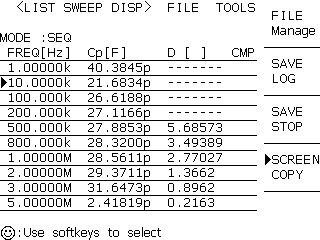
\includegraphics[width=0.5\linewidth]{./images/lcr_ebox_capacitance.jpg}
    \caption{Kapazitätsmessung des E-Box mit dem LCR-Messgerät}
    \label{fig:lcr_ebox_capacitance}
\end{figure}

% ----------------------------------------
% Sec: Versuchdurchführung
% ----------------------------------------
\section{Versuchdurchführung}
\label{sec:versuchdurchfuehrung}

Da die Auswertung der Schmierfilmdicke in dieser Arbeit optisch und elektrisch geschieht wird, ist die Sauberkeit vor dem Beginn einer Messung besonders wichtig zu achten.
Die Glasscheibe, die Kugel, das Kugelsupport und das Ölreservoir müssen vor jeder Messung mit Waschbenzin oder Isopropanol gereinigt werden und dürfen keine Schlieren aufweisen.

Nach der Reinigung können das Support und die Kugel in das Gerät eingesetzt werden.
Die Führung der Kugel wird zuerst in die Ausgangswelle des zweiten Motors eingesteckt und dann auf das Support aufgelegt.
Die Kabel sollen Abstand von den Wände des Reservoirs und der Motorwelle gehalten werden, um ein Unfall (Kurzschluss der Kugel, Verfangen des Kabels) während des Betriebs zu vermeiden.
Die Abbildung \ref{fig:ehd_topf_mit_kugel_und_support} zeigt den Blick von oben des EHD-Prüftopfs mit montierten Support und aufgelegter Kugel bereits für den Versuch.
% ----------------------------------------
% Fig: EHD-Prüftopf mit montierten Support und Modifizierter Kugelführung
% ----------------------------------------
\begin{figure}[htb]
    \centering
    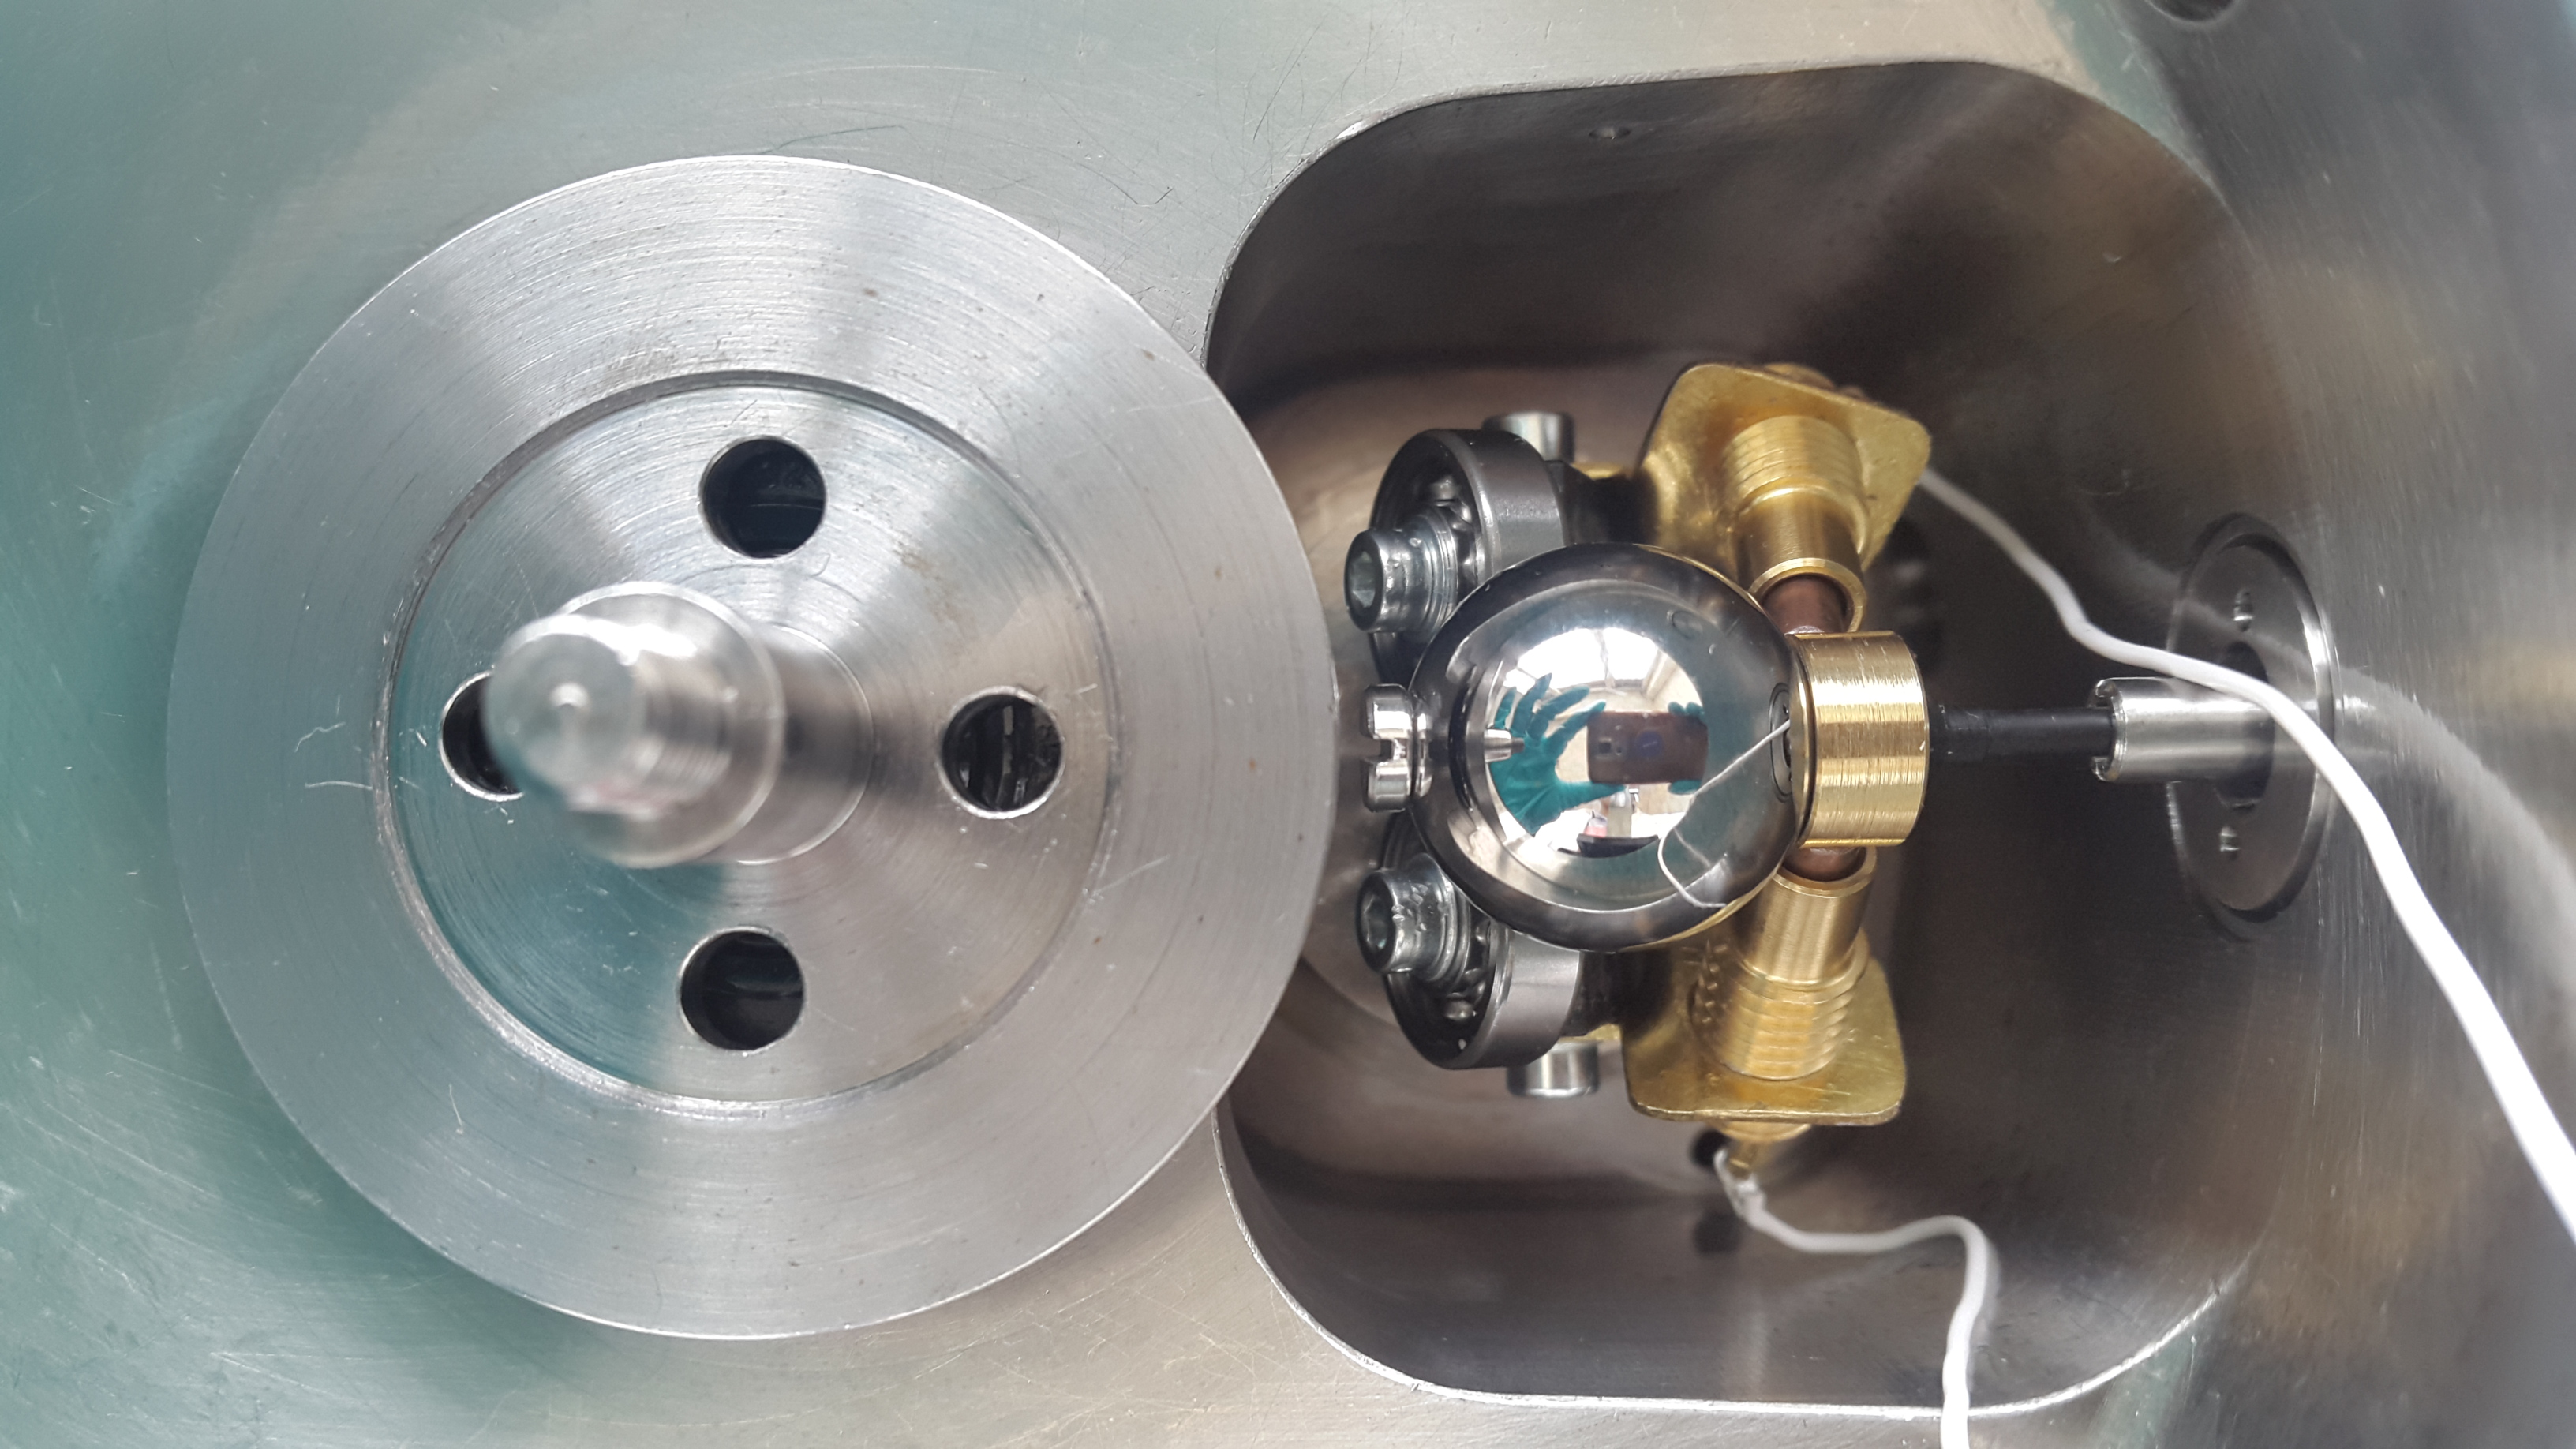
\includegraphics[width=0.7\linewidth]{./images/ehd_topf_mit_kugel_und_support.jpg}
    \caption{Topf des EHD-Geräts mit montierten neuen Kugelsupport und der Modifizierter Kugelführung}
    \label{fig:ehd_topf_mit_kugel_und_support}
\end{figure}

Die Bestimmung des Messpunkts für die optische Messung erfolgt zuerst auf der nicht beschichteten Seite der Scheibe.
Da nach wird die Scheibe \SI{180}{\degree} auf der Cr-Seite gedreht, um der Widerstand der gesamten Messkette (Kabel -> Scheibe -> Kugel -> Kabel) unter einer Last von \SI{20}{\newton} zu vermessen.
Er ist von dem Radius der Fahrspur abhängig und beträgt ungefähr \SIrange{17}{18}{\ohm}.
Die Suche nach dem Messpunkt passiert beim leeren Reservoir, weil ein sauberer Kontakt zwischen Scheibe und Kugel für die Bestimmung der Höhe des Spacer-Layers nötig ist.
Außerdem darf man nur das Spurwechseln beim leeren Zustand machen, weil das Verlaufen des Öles über die Lasteinheit in mechanischen Baukasten zum Schaden führen kann.
Man sollte die Spur von außen nach innen wechseln, um die Entstehung der Insel, die elektronisch zu den Elektroden (Kupferstreifen) isoliert sind, zu vermeiden.
Danach kann man das Öl mit der Hilfe einem Trichter befüllen und den Prüftopf mit dem Deckel zu machen.
Abbildung \ref{fig:ehd_kontakt} zeigt den gut auswertbaren und schlechten EHD-Kontakte an.
% ----------------------------------------
% Fig: Bestimmung des Messpunkts
% ----------------------------------------
\begin{figure}[htb]
    \centering
    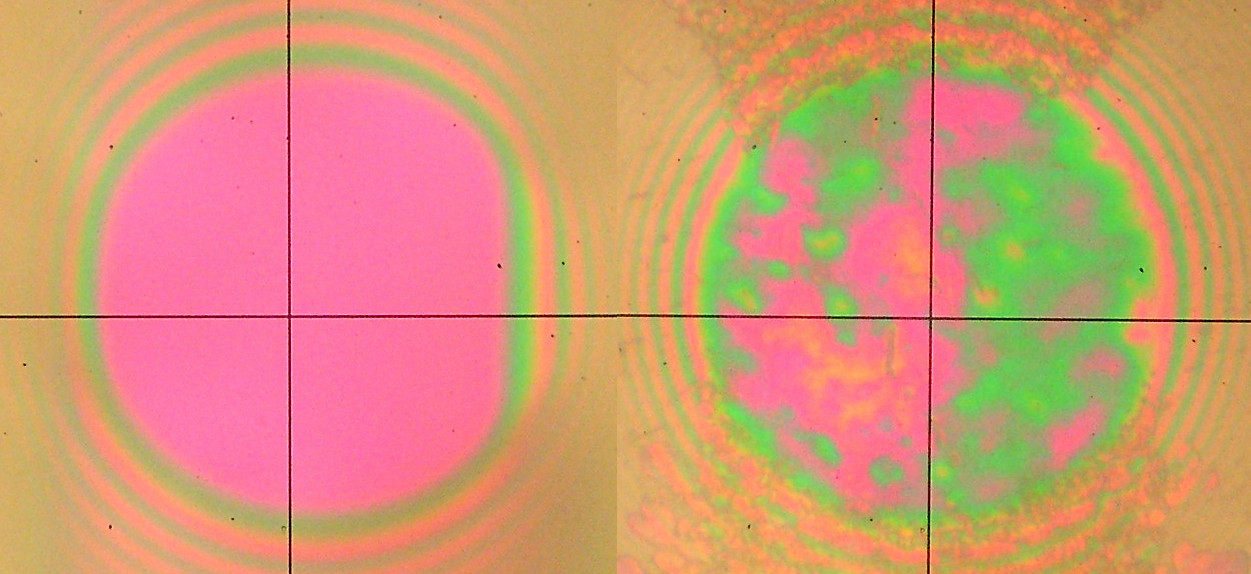
\includegraphics[width=0.7\linewidth]{./images/ehd_kontakt.jpg}
    \caption{EHD-Kontakt: gut auswertbarer Kontakt (links); schlechter Kontakt (rechts) \cite{mach_2008}}
    \label{fig:ehd_kontakt}
\end{figure}

Zur Messung bei Öl-Vollschmierung wird das Ölreservoir bis zur Hälfte der Kugel (ca. \SI{120}{\ml}) gefüllt.
Das Ölbad wird vor jeder Messreihe während des Heizvorgangs (bei \SI{40}{\degreeCelsius}, \SI{60}{\degreeCelsius} und \SI{80}{\degreeCelsius}) für ca. \SI{10}{\minute} durchmischt, um eine homogene Temperatur im Ölbad beim Versuch zu herrschen.
Das genaue Vorgehen einer solchen Messung wurde von \textit{Surborg} in seiner Arbeit \cite{surborg_2007} beschrieben und ist im Anhang zu finden.

Neben dem Widerstand des Kontakts wird die Hintergrund-Kapazität des Prüfstands auch gemessen.
Dieser Wert wird als Störkapazität bezeichnet und soll von der Ergebnissen beseitigt werden.

Die Last von \SI{20}{\newton} wird in Anlehnung an vorherigen Arbeiten gewählt.
Nach dem Abschnitt \ref{sec:betrachtung_des_ehd_kontaktes} lässt es sich für den hier betrachteten Fall eines Kugel-Scheibe-Modells eine maximale Pressung im Kontakt $p_0 =$ \SI{509}{\mega\pascal} berechnen.
Damit liegt der Kontakt im unteren Bereich der EHD-Schmierung.
Diese geringe Last ist gut, somit wird die Gefahr von Beschädigung auf der Scheibe bzw. der Silikatschicht gering gehalten.

Nachdem die Höhe des Spacer-Layers bestimmt wurde, wird die Scheibe ein Stück weiter gedreht und auf etwa \SI[per-mode=symbol]{100}{\mm\per\second} beschleunigt.
Während dieser Einlaufphase wird ständig das Live Bild auf dem SW-Monitor beobachtet.
Sobald sich ein klarer, gut messbarer Verlauf abzeichnet (siehe Abbildung \ref{fig:ehd_live_bild}), kann man mit der Messung begonnen werden.
Wichtig ist, dass man die Messungen zügig machen soll, um die Beschädigung der Chromschicht und Silikatschicht zu vermeiden.
% ----------------------------------------
% Fig: Schlechtes und gutes Live Bild
% ----------------------------------------
\begin{figure}[htb]
    \centering
    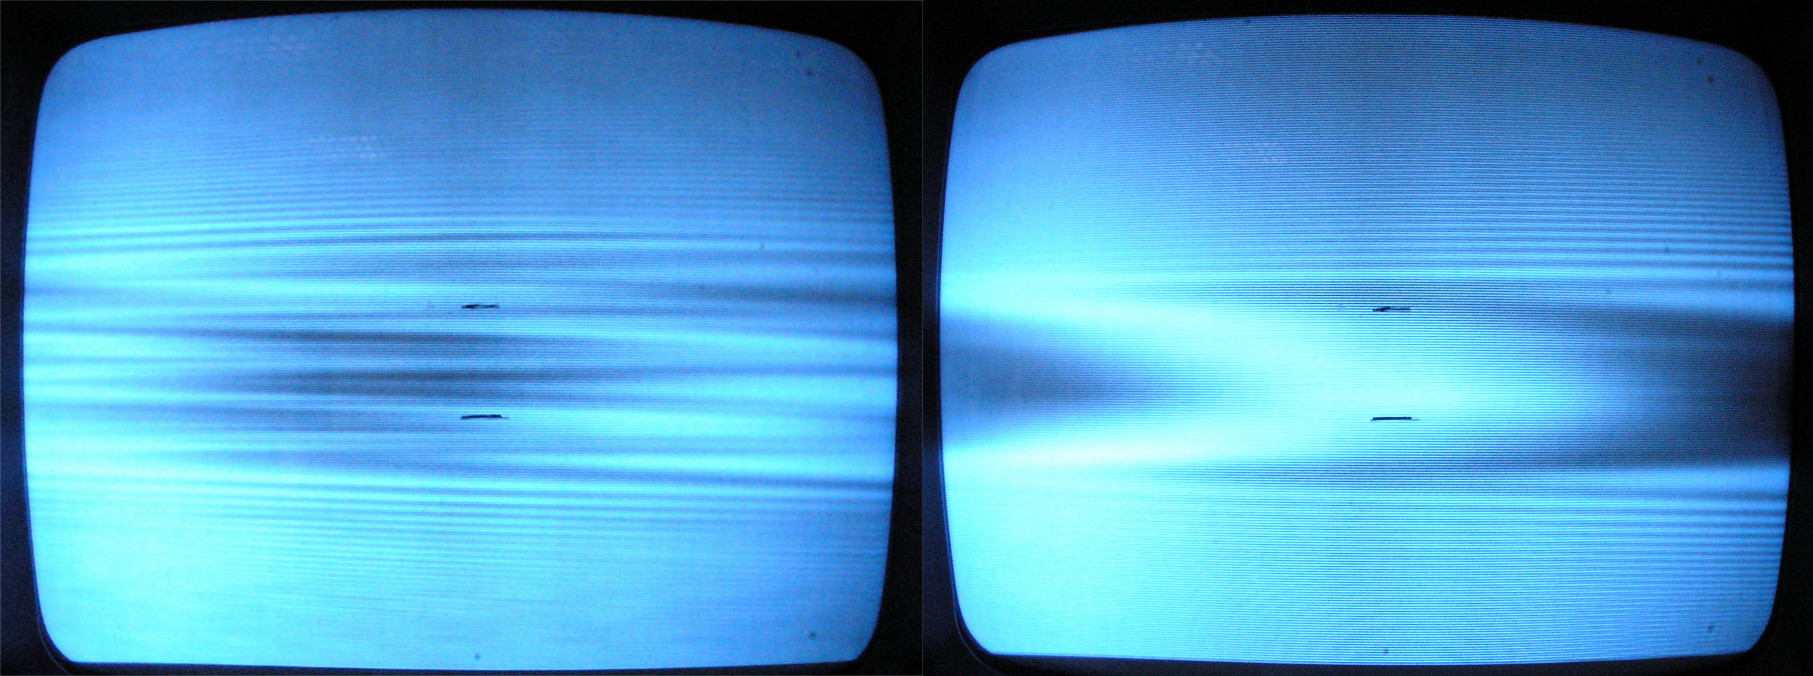
\includegraphics[width=0.8\linewidth]{./images/ehd_live_bild.jpg}
    \caption{Live Bild: nicht verwertbarer Verlauf (links); guter Verlauf (rechts) \cite{mach_2008}}
    \label{fig:ehd_live_bild}
\end{figure}

Die Versuche in dieser Arbeit werden mit den Versuchsparameter (Tabelle \ref{tab:ehd_test_params}) und den Einstellungen des mobilen Messsystems von IMKT (Tabelle \ref{tab:einstellungen_des_ladekurve_messsystems}) wie folgt geplant und durchgeführt:
% ----------------------------------------
% Enum: Versuchsplan
% ----------------------------------------
\begin{enumerate}
    \item Vergleichsmessungen von neu modifizierten Bauteilen (Kugel, Support, Glasscheibe) mit den von \textit{PCS}
    \item Schmierfilmdickenmessung am EHD-Gerät (optisch)
    \item Schmierfilmdickenmessung mit dem mobilen Messsystem von IMKT (elektrisch)
    \item Vergleich der theoretischen Schmierfilmdickenbestimmung mit 2. und 3. zur Überprüfung des Messverfahrens
\end{enumerate}

% ----------------------------------------
% Tab: Versuchsparameters am EHD-Prüfstand
% ----------------------------------------
\begin{table}[htbp]
    \centering
    \caption{Versuchsparameters beim EHD-Prüfstand}
    \begin{tabular}{ll}
        Öl & FVA 3 \\
        Last [\si{N}] & 20 \\
        Temperatur [\si{\degreeCelsius}] & 40 – 60 – 80 \\
        Geschwindigkeit [\si[per-mode=symbol]{\meter\per\second}] & \SIrange[per-mode=symbol]{0.1}{1.4}{\meter\per\second} \\
        Geschw. Stufen [\si{\%}] & 40 \\
        Schlupf [\si{\%}] & 0; 5 \\
    \end{tabular}
    \label{tab:ehd_test_params}
\end{table}


% ----------------------------------------
% Tab: Einstellungen des mobilen Messsystems von IMKT
% ----------------------------------------
\begin{table}[htbp]
    \centering
    \caption{Einstellungen des mobilen Messsystems von IMKT}
    \begin{tabular}{ll}
        Messtyp                          & Anzahl der Messwerte \\
        Anzahl der Messwerte [\si{1}]    & 2500                 \\
        Anzahl der Ladekurven [\si{1}]   & 10                   \\
        Abtastrate [\si{\Hz}]            & 250000               \\
        Ladespannung [\si{\volt}]        & 0.2                  \\
        Verzögerung [\si{\ms}]           & 1                    \\
        Entladezeit [\si{\ms}]           & 100                  \\
        Ladevorwiderstand [\si{\ohm}]    & 1012700              \\
        Störkapazität [\si{\pico\farad}] & 0                    \\
    \end{tabular}
    \label{tab:einstellungen_des_ladekurve_messsystems}
\end{table}





% ----------------------------------------
% Diskussion
% ----------------------------------------
\chapter{Diskussion}
\label{chap:diskussion}


% ----------------------------------------
% Zusammenfassung und Ausblick
% ----------------------------------------
\chapter{Zusammenfassung und Ausblick}
\label{zusammenfassung_und_ausblick}

Was soll in die Zusammenfassung sein.

Was ist der Ausblick von dieser Arbeit


% ----------------------------------------
% Literaturverzeichnis
% ----------------------------------------
\bibliographystyle{unsrt}
\bibliography{./literatures/literaturen}

% ----------------------------------------
% Anhang
% ----------------------------------------
Anhang:

Bilde, Formelherleitung, Zeichnung etc...


\end{document}
